\chapter{Template}
\label{sec:template}

\section{Instructions}

\begin{description}
\item[\textcolor{green}{Author}] Author of the approaches description  \todo{Name -  Company}
\item[\textcolor{blue}{Assessor 1}] First assessor of the approaches \todo{Name - Company}
\item[\textcolor{magenta}{Assessor 2}] Second assessor of the approaches \todo{Name - Company}
\end{description}

In the sequel, main text is under the responsibilities of the author.

\begin{author_comment}
Author can add comments using this format at any place.
\end{author_comment}

\begin{assessor1}
First assessor can add comments using this format at any place.
\end{assessor1}

\begin{assessor2}
Second assessor can add comments using this format at any place.
\end{assessor2}

When a note is required, please follow this list :
\begin{description}
\item[0] not recommended, not adapted, rejected
\item[1] weakly recommended, adapted after major improvements, weakly rejected
\item[2] recommended, adapted (with light improvements if necessary)  weakly accepted
\item[3] highly recommended, well adapted,strongly accepted
\item[*] difficult to evaluate with a note (please add a comment under the table)
\end{description}

All the notes can be commented under each table.

This section defines the criteria for the means and tools dedicated to verification and validation activities, in the WP4 workpackage. 

Criteria of this section are defined according \citep{D4.1}.

\section{Presentation}

This section gives a quick presentation of the approach and the tool.

\begin{description}
\item[Name] \todo{Name of the approach and the tool}
\item[Web site] \todo{if available, how to  find information}
\item[Licence] \todo{Kind of licence}
\end{description}

\paragraph{Abstract} Short abstract on the approach and tool (10 lines max)

\paragraph{Publications} Short list of publications on the approach (5 max)


\section{Common criteria on secondary means and tools}
\label{common}
This section discusses the common criteria of the means and tools according to the project requirements on tools and the results of T7.1.

\subsection{Project and WP2 requirements}

The objectives of this list of criteria is to check if the proposed means and tools meet the main criteria of the project: open-source approaches, usability, modularity, coverage of the objectives,...

According WP2 requirements, give a note for characteristics of the use of the tool (from 0 to 3) :

\begin{tabular}{|l | c | c | c | c|}
\hline
& \textcolor{green}{Author} & \textcolor{blue}{Assessor 1} & \textcolor{magenta}{Assessor 2} & Total \\
\hline 
Open Source (D2.6-02-074) & & & &  \\
\hline 
Portability to operating systems (D2.6-02-075) & & & &  \\
\hline
Cooperation of tools (D2.6-02-076) & & & &  \\
\hline
Robustness (D2.6-02-078) & & & & \\
\hline
Modularity (D2.6-02-078.1) & & & & \\
\hline
Documentation management (D2.6-02-078.02) & & & & \\
\hline
Distributed software development (D2.6-02-078.03)  & & & & \\
\hline
Simultaneous multi-users (D2.6-02-078.04)   & & & & \\
\hline
Issue tracking (D2.6-02-078.05) & & & & \\
\hline
Differences between models (D2.6-02-078.06) & & & & \\
\hline
Version management (D2.6-02-078.07) & & & & \\
\hline
Concurrent version development (D2.6-02-078.08) & & & & \\
\hline
Model-based version control (D2.6-02-078.09) & & & & \\
\hline
Role traceability (D2.6-02-078.10) & & & & \\
\hline
Safety version traceability (D2.6-02-078.11) & & & & \\
\hline
Model traceability (D2.6-02-079) & & & & \\
\hline
Tool chain integration & & & & \\
\hline
Scalability & & & & \\
\hline
User Friendliness & & & & \\
\hline
\end{tabular}



\subsection{Qualification}

This section discusses how the tool can be classified according EN50128 requirements (D2.6-02-085). Some qualification shall be mandatory  if the tool is involved to design a SIL4 software.


\begin{tabular}{|l | c | c | c | c|}
\hline
& \textcolor{green}{Author} & \textcolor{blue}{Assessor 1} & \textcolor{magenta}{Assessor 2} & Total \\
\hline 
Tool manual (D.2.6-01-42.02) & & & &  \\
\hline
Proof of correctness (D.2.6-01-42.03)   & & & & \\
\hline
Existing industrial  usage  & & & & \\
\hline
Model verification & & & & \\
\hline
Test generation & & & & \\
\hline
Simulation, execution, debugging & & & & \\
\hline
Formal proof & & & & \\
\hline
\end{tabular}


Which scope of qualification is expected according EN50128 (section 6.7) ?

Score :
\begin{description}
\item[3] already qualified for this level
\item[2] qualification possible to this level, but some elements shall be provided
\item[0] qualification not recommended for this level
\end{description}


\begin{tabular}{|l | c | c | c | c|}
\hline
& \textcolor{green}{Author} & \textcolor{blue}{Assessor 1} & \textcolor{magenta}{Assessor 2} & Total \\
\hline 
class T1 & & & &  \\
\hline
class T2   & & & & \\
\hline
class T3  & & & & \\
\hline
\end{tabular}

\paragraph{Other elements for tool certification}


\subsection{Complementarity with primary toolchain}

The objectives of this list of criteria is to check if the proposed means and tools can be easily integrated to the primary toolchain.

\subsubsection{Language}


According to the decisions and the propositions of T7.1, how the mean and approach can be adapted to or can complete the chosen language and methods:

\begin{tabular}{|l | c | c | c | c|}
\hline
& \textcolor{green}{Author} & \textcolor{blue}{Assessor 1} & \textcolor{magenta}{Assessor 2} & Total \\
\hline 
SysML  & & & & \\
\hline
Scade method & & & & \\
\hline
EFS language & & & & \\
\hline
B Method & & & & \\
\hline
C language & & & & \\
\hline
\end{tabular}

\paragraph{SysML}
How the means or tools can complete SysML ?


\paragraph{Scade, EFS, Classical B}
How the means or tools can complete the current proposals for formal modeling language ?

\paragraph{C language}
How the means or tools can complete or be adapted to SIL4 software in C language ?

\subsubsection{Tools and platforms}

According to the decisions and the propositions of T7.1, how the mean and approach can be integrated to or can complete the chosen tools and platforms:

\begin{tabular}{|l | c | c | c | c|}
\hline
& \textcolor{green}{Author} & \textcolor{blue}{Assessor 1} & \textcolor{magenta}{Assessor 2} & Total \\
\hline 
Eclipse & & & &  \\
\hline
Papyrus  & & & & \\
\hline
Scade & & & & \\
\hline
EFS tools & & & & \\
\hline
B tools & & & & \\
\hline
\end{tabular}


\paragraph{Eclipse}
How the means or tools can be integrated to the Eclipse platform ?

\paragraph{Papyrus}
How the means or tools can complete  Papyrus ?


\paragraph{Scade, EFS, Classical B}
How the means or tools can complete the current proposals for formal modeling tools ?





\section{VnV Activities}

The VnV activities are described in details in the verification and Validation Plan  \citep{D4.1}.

\begin{figure}[htb]
  \centering
  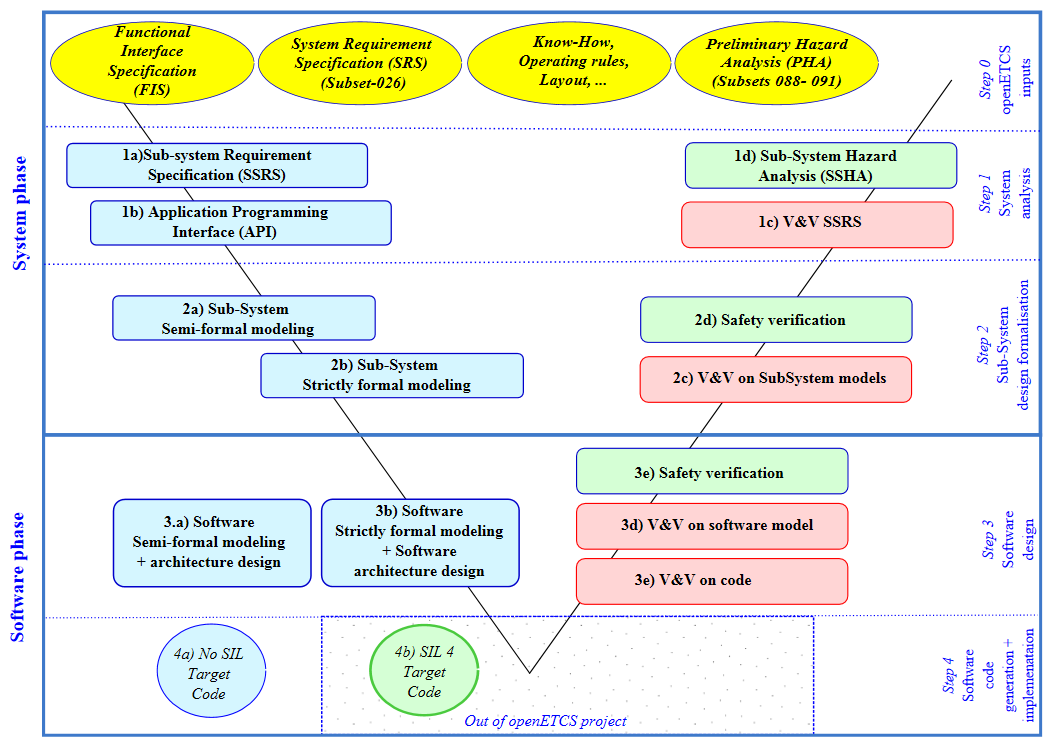
\includegraphics[width=.9\textwidth]{images/ProcessOpenETCS-BeM.png}
  \caption{openETCS Process (rough view)}
  \label{fig:openETCSProcess}
\end{figure}

According figure \ref{fig:openETCSProcess}, for which activities is the mean or tool suitable (see also \citep{D4.1} section 5.1.2 for more details) ?


\begin{tabular}{|l | c | c | c | c|}
\hline
& \textcolor{green}{Author} & \textcolor{blue}{Assessor 1} & \textcolor{magenta}{Assessor 2} & Total \\
\hline 
1c SSRS Verification & & & &  \\
\hline
1c SSRS Validation & & & &  \\
\hline
2c SFM Verification & & & &  \\
\hline
2c SFM Validation & & & &  \\
\hline
3d SW-SFM Verification & & & &  \\
\hline
3d SW-SFM Validation & & & &  \\
\hline
3d SW-FFM Verification & & & &  \\
\hline
3d SW-FFM Validation & & & &  \\
\hline
3e Code Verification & & & &  \\
\hline
3e Code Validation & & & &  \\
\hline
DAS2V Verification \footnote{DAS2V : Design Artifact Subject to Verification and Validation, see \citep{D4.1}}& & & &  \\
\hline
DAS2V Validation & & & &  \\
\hline
\end{tabular}


\section{Properties}

Which kind of properties or elements are verified or validated by the mean or tool (see also \citep{D4.1} section 4)  ?



\begin{tabular}{|l | c | c | c | c|}
\hline
& \textcolor{green}{Author} & \textcolor{blue}{Assessor 1} & \textcolor{magenta}{Assessor 2} & Total \\
\hline 
Functionalities of the system and sub-system & & & &  \\
\hline
System and sub-system architecture & & & &  \\
\hline
External and internal interfaces of sub-system & & & &  \\
\hline
Software components & & & &  \\
\hline
Performance constraints & & & &  \\
\hline
Safety objectives & & & &  \\
\hline
Functional properties & & & &  \\
\hline
Safety properties & & & &  \\
\hline
\end{tabular}



\section{Verification methods and tools}

Which kind of methods is proposed (see also \citep{D4.1} section 5.3) ?



\begin{tabular}{|l | c | c | c | c|}
\hline
& \textcolor{green}{Author} & \textcolor{blue}{Assessor 1} & \textcolor{magenta}{Assessor 2} & Total \\
\hline 
Reviews & & & &  \\
\hline
Inspections & & & &  \\
\hline
Software Architecture Analysis Method & & & &  \\
\hline
Architecture Tradeoff Analysis Method & & & &  \\
\hline
Model-Based System Integration Testing & & & &  \\
\hline
Model-Based Testing of Generated High-Level Code & & & &  \\
\hline
Abstract Interpretation & & & &  \\
\hline
Deductive Verification & & & &  \\
\hline
Model Checking & & & &  \\
\hline
Correct by Construction Formal Methods & & & &  \\
\hline
Verification with Formal Methods & & & &  \\
\hline
Simulation-based & & & &  \\
\hline
\end{tabular}

\section{Validation means and tools}

The following list of criteria focuss on means and tools to support validation activities, according WP2  requirements :

\begin{tabular}{|l | c | c | c | c|}
\hline
& \textcolor{green}{Author} & \textcolor{blue}{Assessor 1} & \textcolor{magenta}{Assessor 2} & Total \\
\hline 
Simulation-based & & & &  \\
\hline
Step-by-step simulation (D2.6-01-036) & & & &  \\
\hline
Environment emulation (D2.6-01-037 and D2.6-02-080) & & & &  \\
\hline
Time-based test case (D2.6-02-081) & & & &  \\
\hline
Test cases writing (D2.6-01-038) & & & &  \\
\hline
Test cases execution (D2.6-01-038) & & & &  \\
\hline
Test cases storage (D2.6-01-038) & & & &  \\
\hline
Version management of test cases (D2.6-02-082) & & & &  \\
\hline
Test generation from independant test model (D2.6-02-083) & & & &  \\
\hline
Test sequences writing (D2.6-02-084) & & & &  \\
\hline
Test sequences execution (D2.6-02-084) & & & &  \\
\hline
Test sequences storage (D2.6-02-084) & & & &  \\
\hline
\end{tabular}

\section{Other Criterias}



\begin{comment}
MPD : Todo
Ideas welcomed !

\end{comment}





\section{Other comments}



\begin{comment}
This section is available for the author or the assessors to  complete the description and criteria.
\end{comment}



